\qns{Image Restoration}
\newline
\newline
Finally! You did it!! After years of trying you finally got the perfect shot of the campanile. You were so excited you decided you should post it on Instagram. But first, you wanted to share it with your friends. You called them over and showed it to them. Your friends are from Stanford. They thought it would be cool to play a trick on you, so they edited your picture by adding the text `` I wish I was at Stanford though! :( ". 

\begin{figure}[h]
\centering
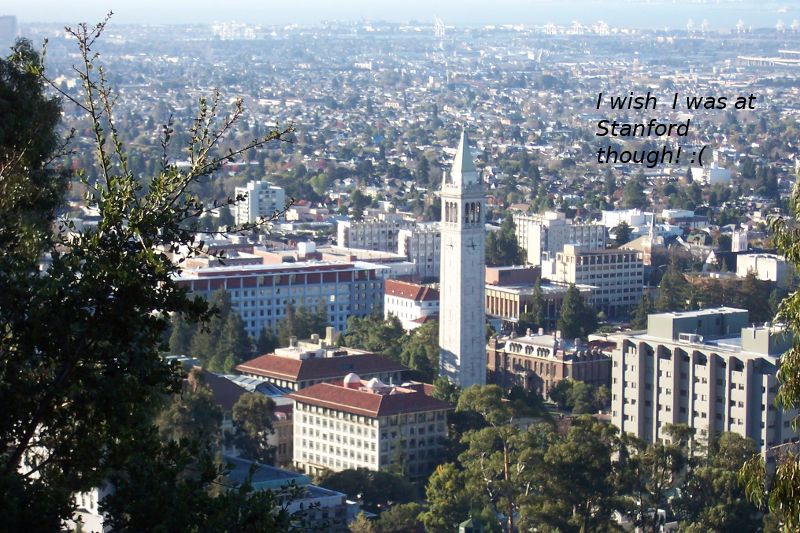
\includegraphics[scale=2.00]{figures/campanile_img_corrupted.jpg}
\caption{Your perfect shot corrupted by your Stanford friends :(}
\end{figure}
You see this in the morning, and realize you had no backup of your photo. While the prank was in good fun, you would like to get your original image back. So, you apply your Berkeley smarts in order to recreate the original image. You will be completing an exercise to try to restore the image your friends corrupted.
\newline
\newline
First, we will need to understand the representation an image (grayscale) stored in memory as a discrete sampling of a function over a continuous domain. One can think of an image as a function $f(x,y)\colon \Omega \subset  \mathbb{R}^{2}\to \mathbb{R}_{+}$.  The range represents the color intensity at each point in the image.
\newline
\newline
To make the definition more concrete, we choose $\Omega = \{(x,y): 1 \leq x \leq W+1,1 \leq y \leq H+1 \}$. Also in practice, the range of the function $f$ may be restricted to the set $[0,255]$, with $0$ being black, $255$ being white, and the numbers in between being various shades of gray going from dark to light. 
\newline
\newline
When we store the image in memory, we sample this function at discrete points and store these samples (typically as a matrix). Given a fixed matrix with $W$ rows and $H$ columns. We may denote the sampled version of the function as: $F(i,j), \hspace{5pt} i \in {1,2, \hdots , W}, \hspace{5pt} j\in {1,2, \hdots , H} $. 
\begin{enumerate}
    \item {[Few lines of justification]}
     To sample an image and ensure that we cover the domain, we may partition the domain into equal sized intervals and sample a point from each interval. One way to do this is to partition the interval of $x$ values over the domain into intervals of width $1$ and to partition the interval of $y$ values of width $1$. We may then sample points on the left boundary of each sub-interval. Given this assumption, explain why it makes sense that $F(i,j) = f\left( i, j\right), \hspace{5pt} i \in {1,2, \hdots , W}, \hspace{5pt} j\in {1,2, \hdots , H}$.
    \newline
    
    \sol{\input{image_restoration_solution/1.1.tex}}
    
    \item {[Single line expression]}
    To solve our problem, it will be useful to approximate the gradient of the function $f$. Recall that the gradient $\nabla f(x,y) = \left[\frac{\partial f(x,y)}{\partial x},\frac{\partial f(x,y)}{\partial y} \right]$. For some small increment $h$, we may approximate it using:
    \begin{align*}
        \frac{\partial f(x,y)}{\partial x} \approx \frac{1}{h} (f(x+h,y) -f(x,y) ) \\
        \frac{\partial f(x,y)}{\partial y} \approx \frac{1}{h} (f(x,y+h) -f(x,y) )
    \end{align*}
    
    Derive an expression for the gradient of $F$,  $\nabla F(i,j) = G(i,j)$ , based on $F$, for  $ i \in \{1,2, \hdots , W-1 \}, \hspace{5pt} j\in \{1,2, \hdots , H-1 \}$, using the approximation above. You may assume step-size $h = 1$.
    \newline
    
    \sol{\input{image_restoration_solution/1.2.tex}}
    
    \item {[Optimization Problem Expression]}
    To solve our problem, we will also assume that we have an idea of which pixels i.e. $(x,y)$ locations were corrupted by Oski's friends (indeed). We will denote this set $\mathcal{A}$, and it's discrete analog as $A$ ($(i,j)$ locations). One way to formulate the problem we are trying to solve is to try to create a new image $f^{*}$ such that over all functions $\hat{f} \colon \Omega \subset  \mathbb{R}^{2}\to \mathbb{R}_{+}$, $f^{*}$ is the solution to:
    \begin{equation*}
          \underset{\begin{subarray}{c}
      \hat{f} \\
      \hat{f}(x,y) = f(x,y)\\
      \forall (x,y) \hspace{5pt} \notin \hspace{5pt} \mathcal{A}
      \end{subarray}}{\text{min }} \int \int_{\Omega} ||\nabla \hat{f}(x,y)||_2 \hspace{5pt}  dx \hspace{2pt} dy
    \end{equation*}
    Intuitively, the idea here is that we want to find the best approximation to the signal, by keeping the values where we know it is not corrupted, but allowing the values in corrupted areas to change, subject to those values not changing too much from their uncorrupted neighbors (hence the gradient term). What we should expect to happen is that the values at the corrupted pixels will be a smoothing of neighboring uncorrupted pixel. However, since we do not store the image as a continuous function, we will have to solve a discrete approximation to the problem above.
    \newline
    Denoting $\Omega$ as the region $a \leq x \leq b, \hspace{5pt} c \leq y \leq d$ for scalars $a,b,c,d$, we may re-write the integral above as 
    \begin{equation*}
        \int_{c}^{d} \int_{a}^{b} ||\nabla \hat{f}(x,y)||_2 \hspace{5pt}  dx \hspace{2pt} dy
    \end{equation*} 
    
    If we partition the interval $[a,b]$ into $m$ equal sub-partitions and $[c,d]$ into $n$ equal sub-partitions, we may then approximate this integral by using a Riemann sum as
    
     \begin{equation*}
        \sum_{i=1}^{m} \sum_{j=1}^{n} ||\nabla \hat{f}(x_{i},y_{j})||_2 \hspace{5pt}  \Delta x \hspace{2pt} \Delta y
    \end{equation*} 
    with $a=x_{1}, < x_{2}, \hdots, < x_{m+1} = b, \hspace{5pt}$
    $c=y_{1}, < y_{2}, \hdots, < y_{n+1} = d, \hspace{5pt} \Delta y = \frac{b-a}{m}, \hspace{5pt} \Delta x = \frac{d-c}{n}$.
    
    Write explicitly a discrete approximation to the optimization problem above in terms of $\hat{F},A, H$ and $W$. (You should ignore terms at the right-most boundaries of your estimate since, the gradient is not computed there. $\hat{G} = \nabla \hat{F} \in \mathbb{R}^{(H-1) \times (W-1)}$).
    
    
    \sol{\input{image_restoration_solution/1.3.tex}}
    
    \item {[Optimization Problem Expression]}
    Show that your formulation can be written as an SOCP (second order cone program).
    \newline
    
    \sol{\input{image_restoration_solution/1.4.tex}}
    
    \item 
    We will implement this in cvxpy.  cvxpy has a function ``cv.tv($\hat{F}$)", which when given a matrix $\hat{F}$, return the approximation of the objective function. 
    \newline
    \newline
    For the constraints we will take the following approach:
    Let the matrix $A$, be as follows:
    \begin{equation*}
        A(i,j) = 
        \begin{cases}
          0 & \text{if } F(i,j) \text{ corrupt}\\
          1 & \text{otherwise}\\
        \end{cases} 
    \end{equation*}
    Then we may write the constraint as $A \circ \hat{F} = A \circ F$, where $\circ$, known as the Hadamard product denotes element wise multiplication of the matrices. 
    \newline
    \newline
    This can be done in cvxpy as:
    \newline
    \newline
    constraints = [cvxpy.multiply(A, $\hat{F}$) == cvxpy.multiply(A, $F$)].
    \newline
    \newline
    Implement this in the Ipython notebook by completing the required portions of the code and test it on the sample images. The matrix $A$ has already been supplied for you. Does is it work? Is there a scenario where this formulation would?
    \newline
    \sol{\input{image_restoration_solution/1.5.tex}}
\end{enumerate}